\subsection{The limit is usable; the horizon matters, not the resolution}
\label{sec:usable-limit}

\begin{figure*}[t]
    \centering
    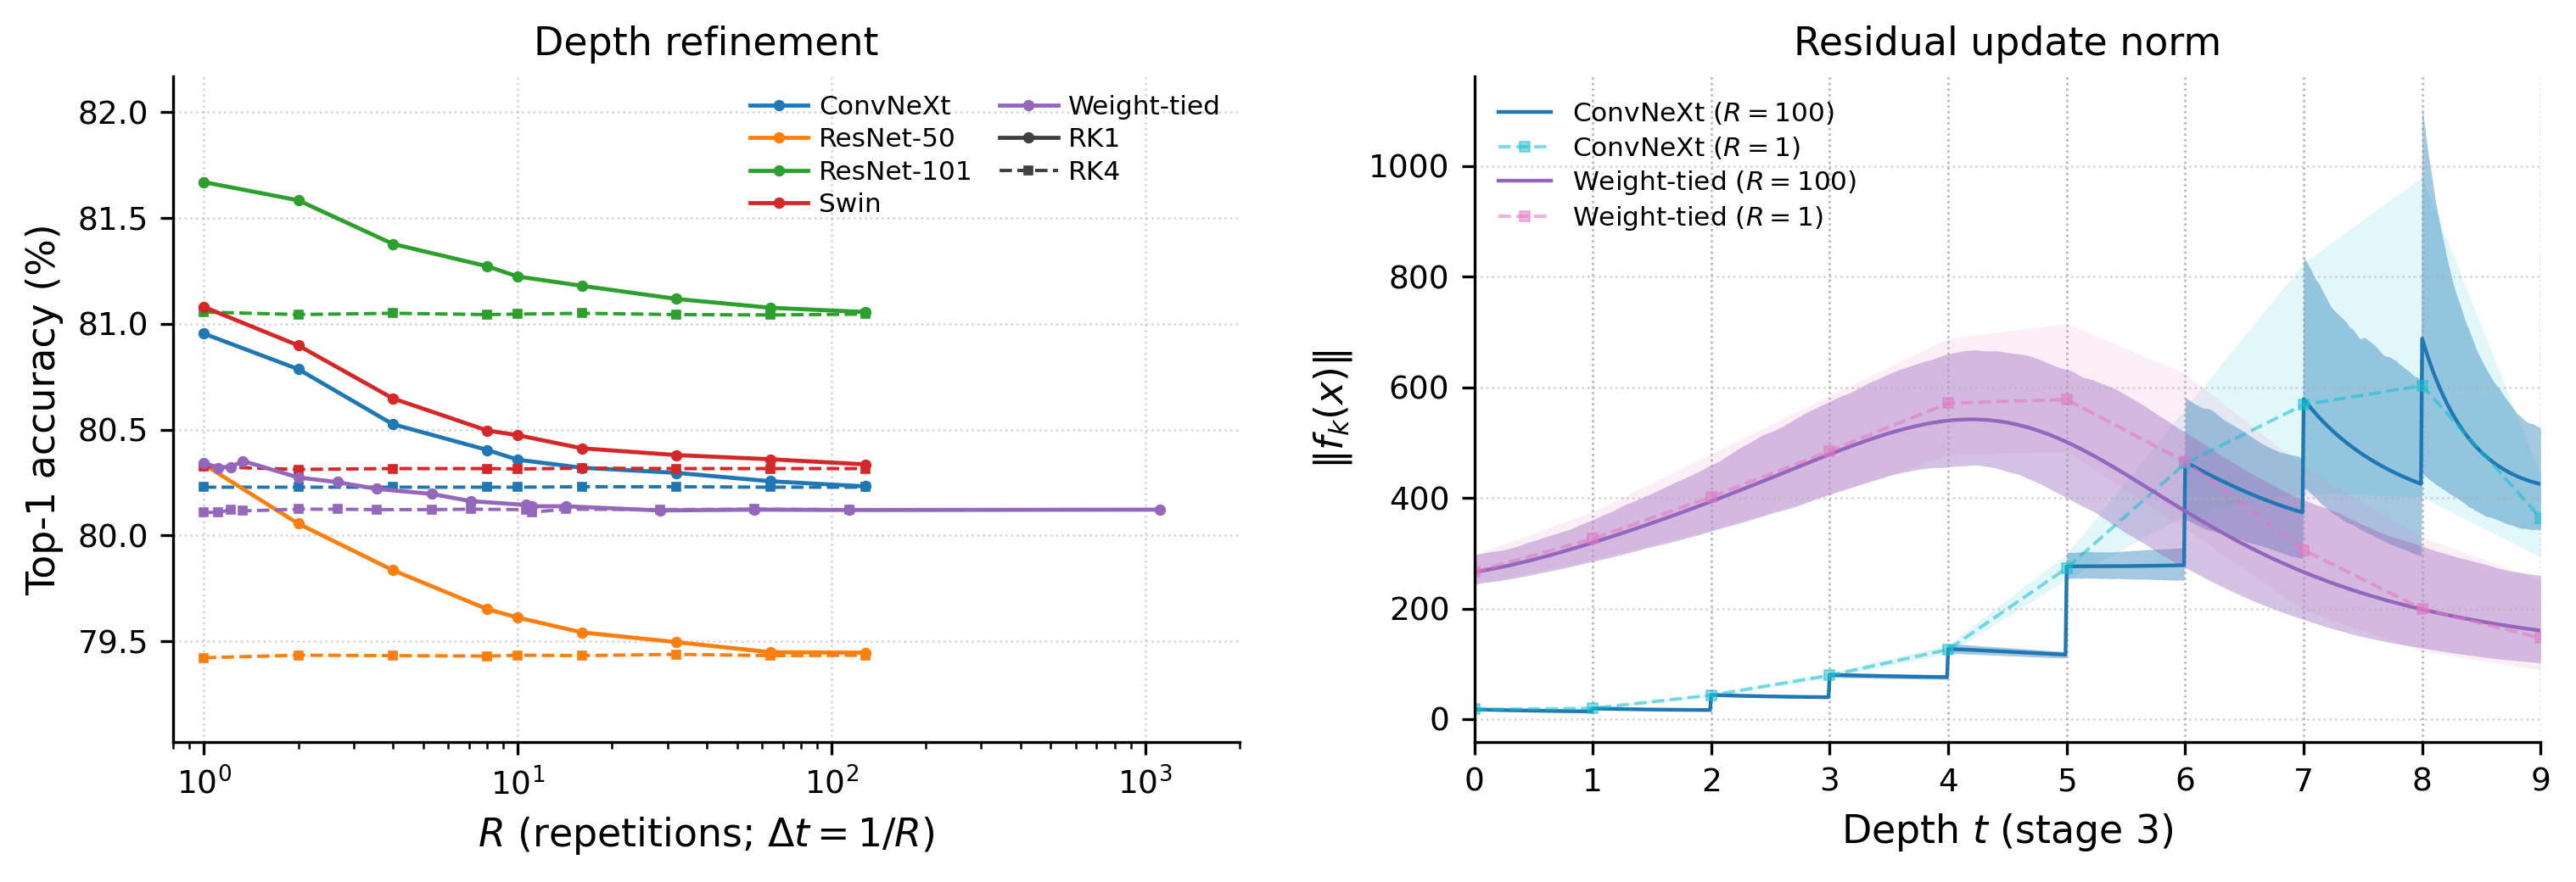
\includegraphics[width=\textwidth]{figures/teaser.png}
    \caption{\textbf{Left:} top-1 against repetitions $R$ (solid: Euler; dashed: RK4),
    with $\Delta t{=}1/R$ so that $T{=}n$ is kept
    (weight-tied: $nR$ applications of the shared block).
    \textbf{Right:} residual norm $\|f(x)\|$ along stage~3
    (mean and P5--P95 over 500 images). The untied field is piecewise constant in
    depth; the weight-tied model is a single smooth autonomous field.}
    \label{fig:refinement}
\end{figure*}

\begin{table}[t]
    \centering
    \caption{Euler refinement with $\Delta t{=}1/R$ ($T$ kept), ImageNet top-1 (\%).
    For the weight-tied model $R$ means $9R$ applications of the shared block.
    ODE limit: RK4 at $R{=}128$ (tied: $1024$ steps).}
    \label{tab:r-ablation}
    \small
    \setlength{\tabcolsep}{2.8pt}
    \resizebox{\linewidth}{!}{%
    \begin{tabular}{lrrrrr}
        \toprule
        $R$ ($\Delta t$) & CNX-T & Swin-T & R-50 & R-101 & Tied \\
        \midrule
        $1$ ($1$)       & \accUntied & \accSwin & \accRFifty & \accROneOhOne & \accTied \\
        $2$ ($0.5$)     & 80.78 & 80.90 & 80.06 & 81.58 & 80.27 \\
        $4$ ($0.25$)    & 80.52 & 80.65 & 79.84 & 81.38 & 80.21 \\
        $10$ ($0.1$)    & 80.36 & 80.47 & 79.61 & 81.22 & 80.13 \\
        $32$ ($0.03$)   & 80.29 & 80.38 & 79.50 & 81.12 & 80.11 \\
        $128$ ($0.008$) & 80.24 & 80.34 & 79.45 & 81.06 & \odeTied \\
        \midrule
        ODE limit       & \odeUntied & \odeSwin & \odeRFifty & \odeROneOhOne & \odeTied \\
        Gap ($R{=}1\!\to$ODE) & $-\gapUntiedODE$ & $-\gapSwinODE$ & $-\gapRFiftyODE$ & $-\gapROneOhOneODE$ & $-\gapTiedODE$ \\
        \bottomrule
    \end{tabular}%
    }
\end{table}

We refine our ConvNeXt-T and weight-tied ConvNeXt-T, and the torchvision Swin-T
(\texttt{IMAGENET1K\_V1}), ResNet-50 and ResNet-101 (\texttt{IMAGENET1K\_V2})
(\cref{fig:refinement}, left; \cref{tab:r-ablation}).
All models are evaluated on the full validation set with one transform (resize to $256$,
bilinear, centre crop $224$), so the torchvision models score slightly differently from
their reported $81.47$, $80.86$ and $81.89\%$, which use their own resize.
Accuracy decreases monotonically with $R$ and plateaus at a limit that Euler,
Midpoint and RK4 share once the step is fine enough (\cref{app:solvers}); the
endpoints themselves agree to within $0.25^\circ$ (\cref{app:solver-endpoints}).
The limit costs $\gapTiedODE$ to $\gapRFiftyODE$ points.
The native network is the best point of every sweep and is \emph{not} at the limit:
RK4 with the nine native unit steps already lands on it.
The decoder is tuned to the state produced by one Euler step of size $1$, not to the
flow that step approximates.

Repeating blocks without shrinking the step ($R{=}10$ or $100$ with $\Delta t{=}1$)
collapses every model to $0.10$--$1.03\%$ top-1, and the weight-tied network collapses
in the same way when $T$ leaves the trained horizon (\cref{app:solvers}), as recurrent
networks iterated past their training depth do~\citep{bansal2022endtoend}.
Even $R{=}3$ with $\Delta t{=}1$ ($T{=}27$) drops ConvNeXt-T to $41.0\%$.
With large steps at $T{=}9$ the tied model needs a higher-order solver: with $4$
steps, RK4 reaches $78.9\%$ and Euler $67.8\%$.
Those coarse steps evidence the horizon; they are not a general compute advantage of
the tied stage (\cref{app:solvers}).
